\documentclass[A4]{article}
\usepackage{graphicx}
\usepackage[hidelinks]{hyperref}
\usepackage{wrapfig}
\usepackage{xcolor}

\renewcommand{\familydefault}{\sfdefault}

\pagenumbering{gobble}

\hypersetup{
	colorlinks,
	linkcolor={red!50!black},
	citecolor={blue!50!black},
	urlcolor={blue!80!black}
}

\begin{document}
	\title{Usages of Film Grain}
	\date{}
	
	\maketitle
	
	\section*{What is film grain?}
	\textit{Film grain} is a post-processing effect that overlays the screen with a random noise. In the Unreal Engine 4, it can be tweaked via the \textit{Grain Intensity} parameter. Another random noise function is \textit{Grain Jitter} which changes the movement of the pixels.
	\begin{wrapfigure}{r}{0.5\textwidth}
		\begin{center}
			\vspace{-20px}
			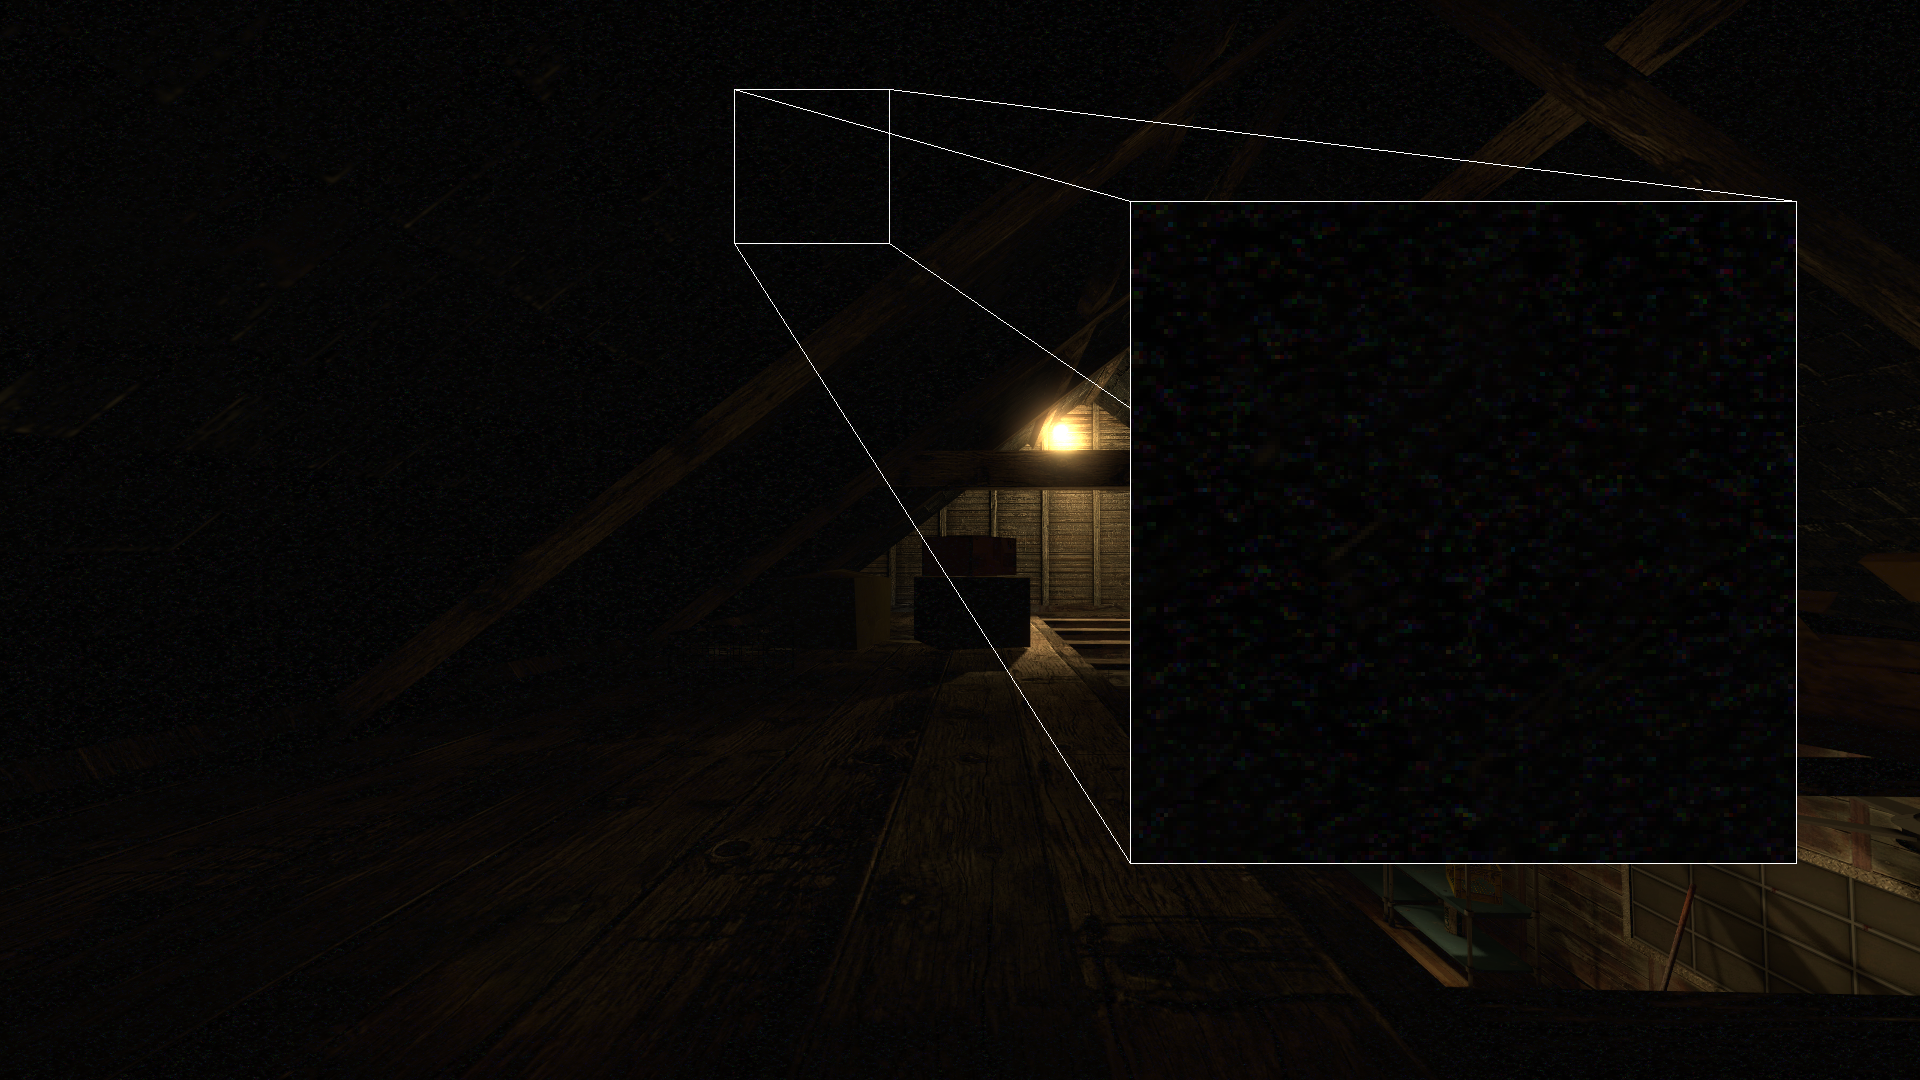
\includegraphics[scale=0.1]{Estranged.png}
			\vspace{-20px}
		\end{center}
		\caption{Film noise in \textit{Estranged: Act 1}. The noise is only present in dark areas.}
		\vspace{-20px}
	\end{wrapfigure}
	Note that the Unreal Engine 4 effect emulates film \textit{grain}, not film \textit{noise} as the grain is present everywhere, whereas the noise only appears in shadowy areas.\\
	It should be also noted that this effect is dynamic. As this is, the images presented here can just offer a first impression. Additionally, the fine details can't be seen accurately in the downscaled images.
	
	\section{Parameters}
	\subsection{Grain Intensity}
	\textit{Grain Intensity} affects the color deviation of the original color, but just the luminance is being affected, the hue stays the same.
	\begin{wrapfigure}{r}{0.5\textwidth}
		\begin{center}
			\vspace{-20px}
			
\includegraphics[scale=0.15]{GrainComparison.png}
			\vspace{-30px}
		\end{center}
		\caption{Comparison of \textit{Grain Intensity}: \textbf{0.0} (right) and \textit{Grain Intensity}: \textbf{1.0}.}
	\end{wrapfigure}
	%\vspace{10px}
	Starting at a value of ~0.15, the noise becomes visible. At 0.37, it gets quite visible with the image getting more and more noisy with an increasing value.
	
	\subsection{Grain Jitter}
	\textit{Grain Jitter} affects the movement of the pixels. As the effect is pretty unobtrusive, it first comes visible at high values as 5.
	\begin{wrapfigure}{r}{0.5\textwidth}
		\begin{center}
			\vspace{-20px}
			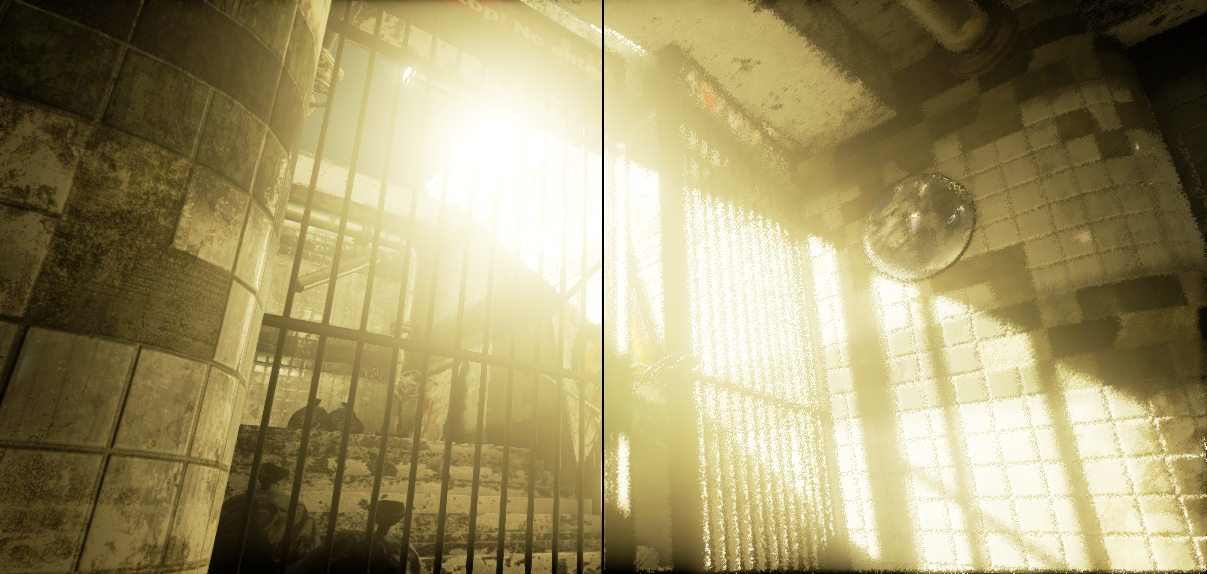
\includegraphics[scale=0.15]{JitterComparison.png}
			\vspace{-20px}
		\end{center}
		\caption{Comparison of \textit{Grain Jitter}: \textbf{0.0} (right) and \textit{Grain Jitter}: \textbf{10.0}. Level: "Reflections" by Epic Games.}
	\end{wrapfigure}
	The edges are getting blurred. Note that the effects blurs mostly into the lower left corner, leading to streaks at the lower and left border when using high values. You can also see that bloom is not affected by \textit{Grain Jitter} - this contrast could be used for interesting effects.
	
	\section{Usage}
	\subsection{Extreme values}
	As always, those values have to be directly typed into the parameter box as the sliders present just support values up to 1.0.
	
	\subsubsection{Extreme Grain Intensity values}
	At high \textit{Grain Intensity} values, the image becomes extremely troubled and confusing. Additionally, a posterization can be seen as the luminace values tend to be complete black or white.
	
	\subsubsection{Extreme Grain Jitter values}
	At high \textit{Grain Jitter} values, the image becomes confusing and distorted. At the lower and left border, streaks get visible. A temporary usage for this effect could be useful as the image can fly apart and assemble right back.
	
	\clearpage
	
	\subsection{Emulation of real cameras}
	In many games, especially in the horror genre, it is not unusual to directly emulate a camera, making the player feel looking through an actual camera.
	\begin{wrapfigure}{r}{0.5\textwidth}
		\begin{center}
			\vspace{-20px}
			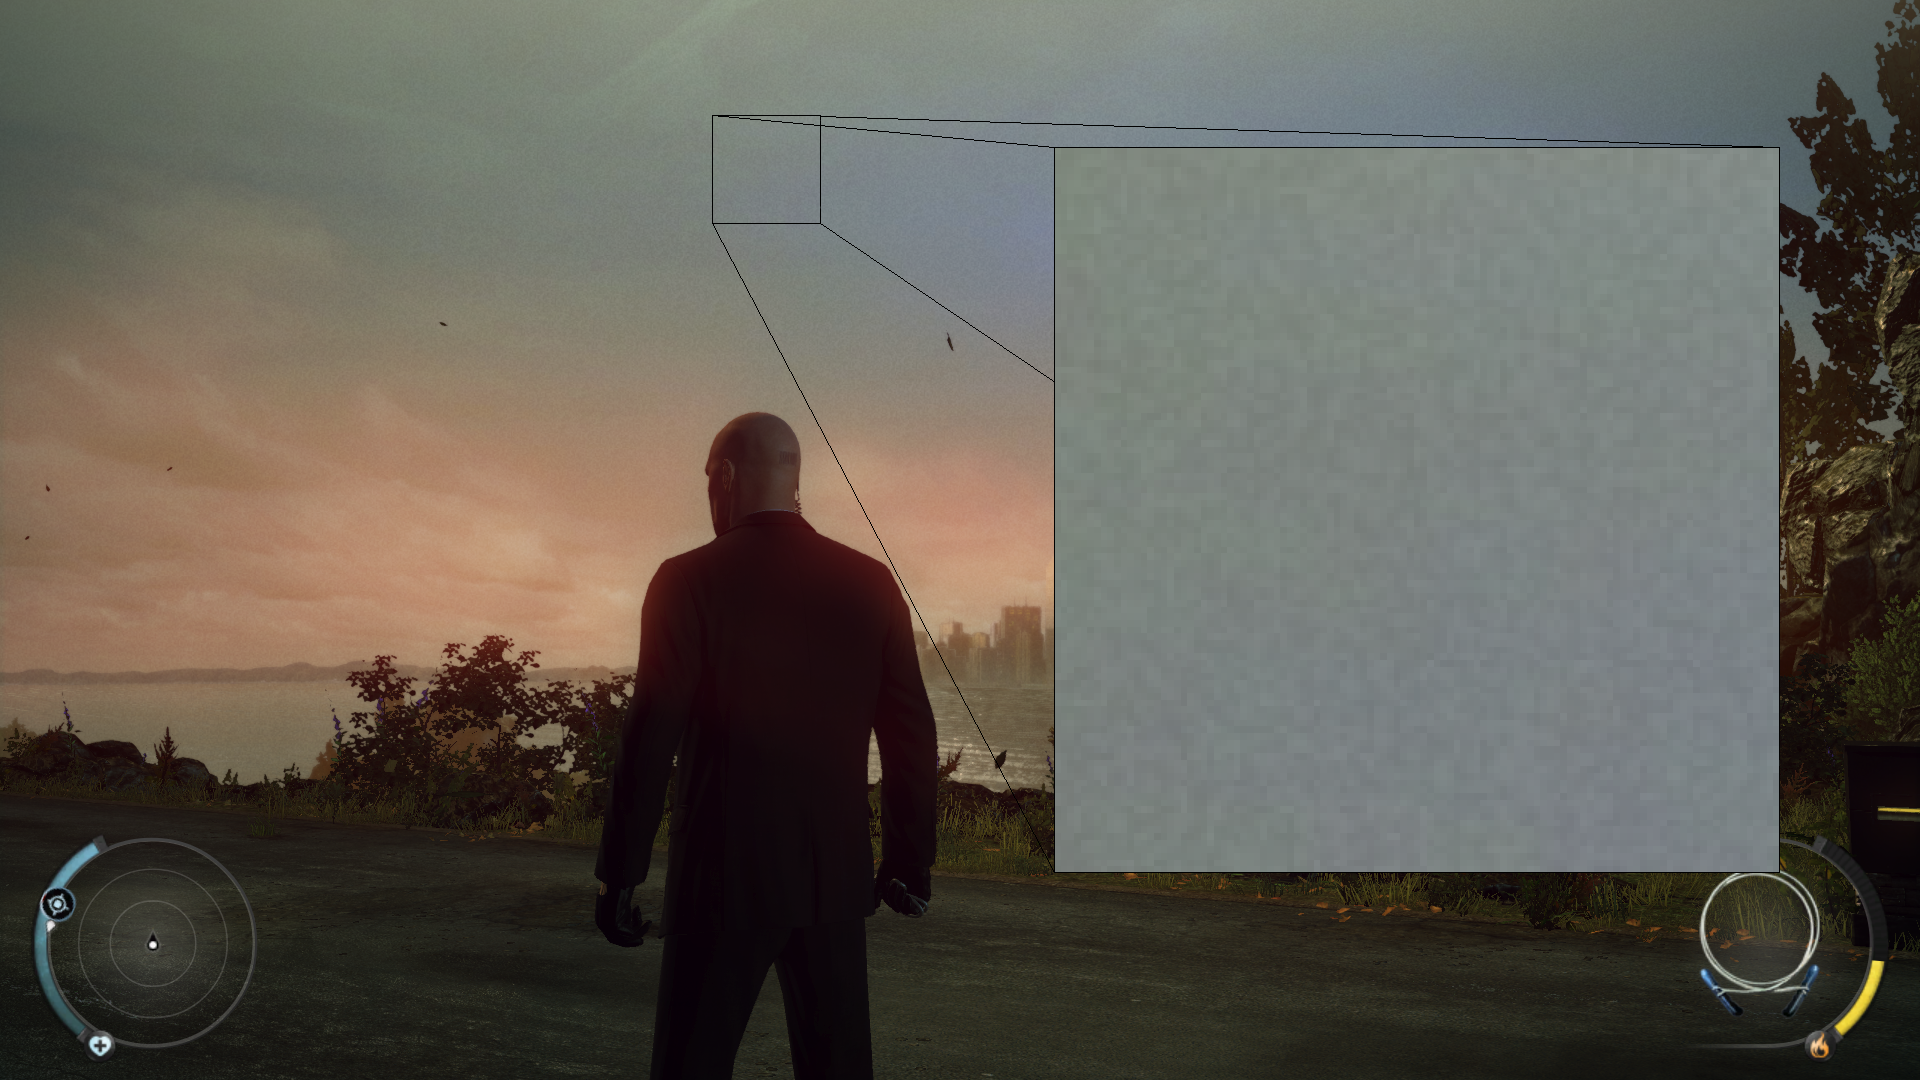
\includegraphics[scale=0.12]{Hitman.png}
			\vspace{-20px}
		\end{center}
		\caption{Film Grain in \textit{Hitman: Absolution}.}
		\begin{center}
			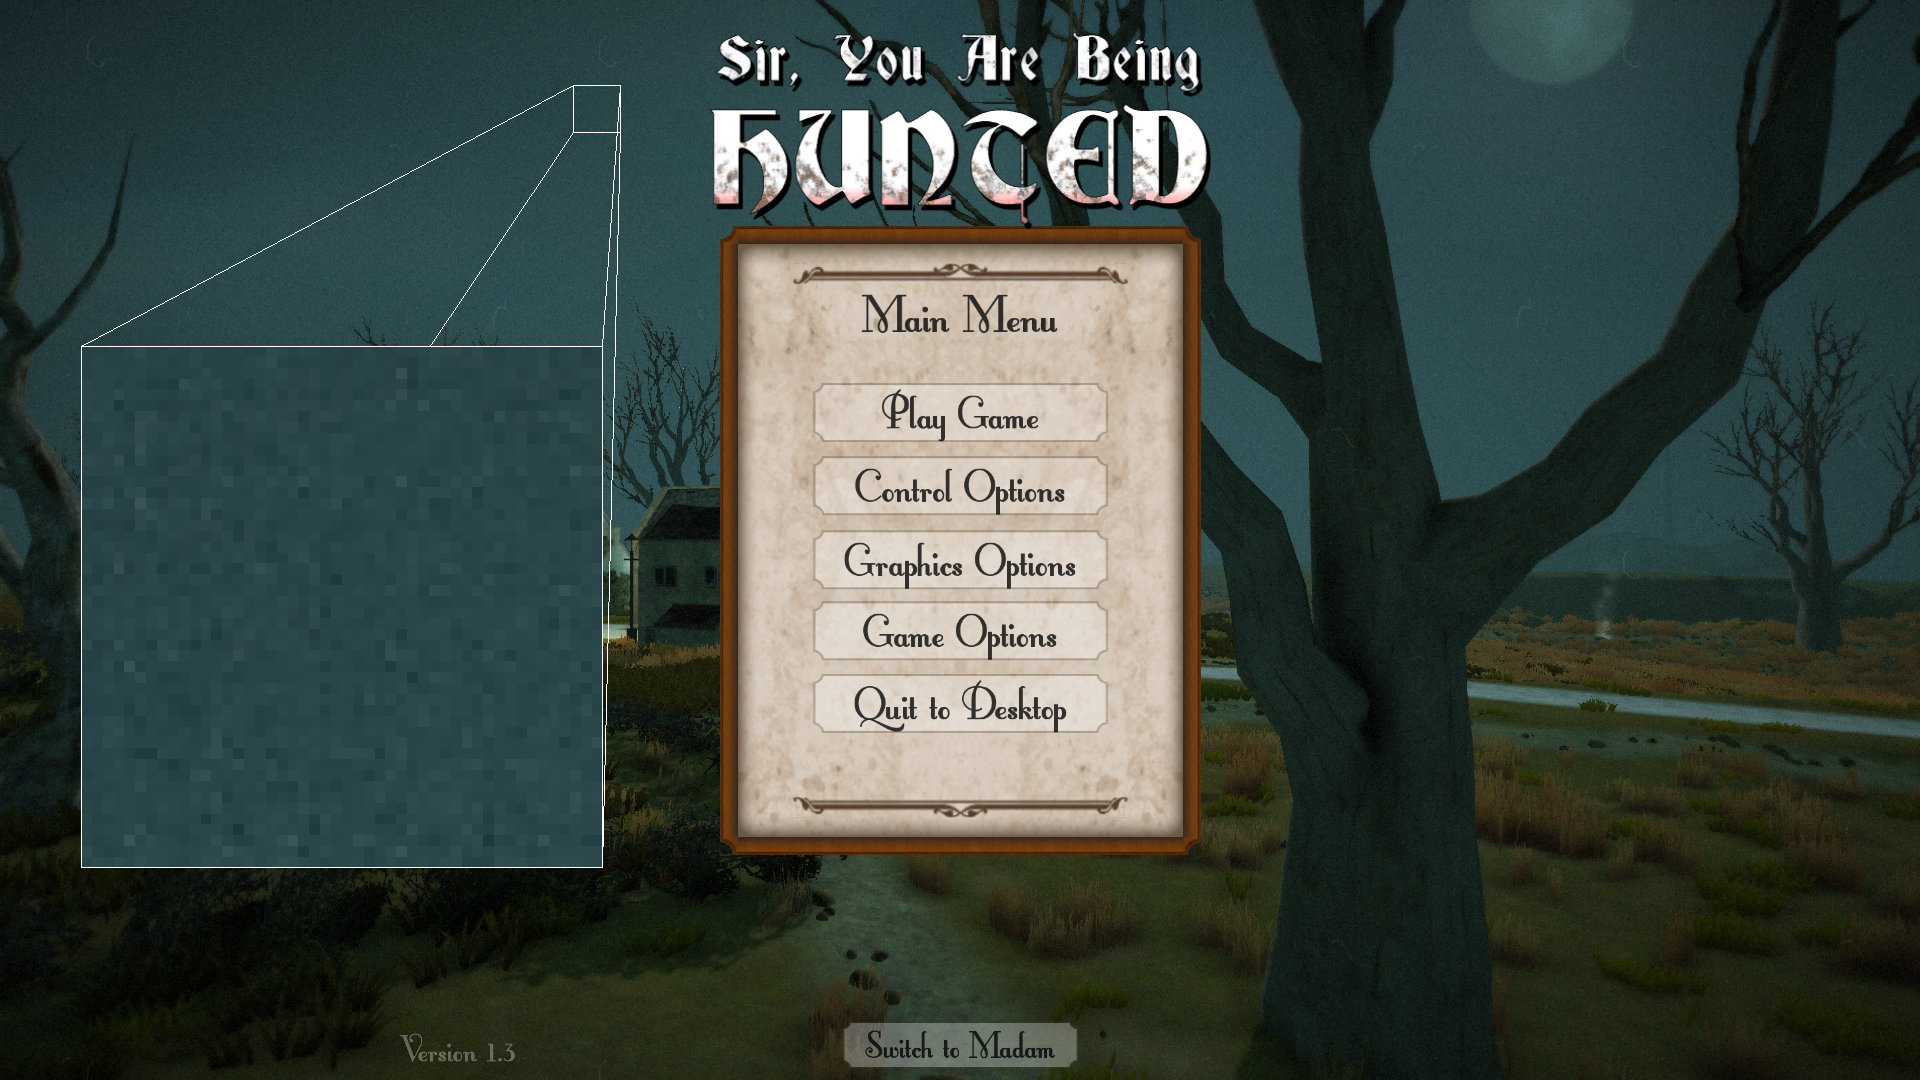
\includegraphics[scale=0.12]{SirYouAreBeingHunted.png}
			\vspace{-20px}
		\end{center}
		\caption{Film Grain in \textit{Sir, You Are Being Hunted}. This effect is only visible in the main menu.}
	\end{wrapfigure}
	Often, this goal is achieved by showing icons in the HUD and other effects, including film grain. Because the simulated camera is often of low quality and the environment is dark, the film grain can be stressed even further.
	
	\subsection{Reducing banding}
	Banding is an effect that appears at fine color gradients where the color gradation is clearly visible. To reduce this, film grain can be used as a replacement for dithering. A similar technique, called Mezzotint, was already used in the middle age to create high-quality prints. However, the film grain should not be used too excessively.
	
	\subsection{Obstructing view}
	Heavy noise obstructs the player's view, makes it harder to focus on enemies, lets the environment appear more confusing and impedes navigation. Therefore, this can be used to illustrate stress situations or also a technology-oriented version of a health bar.
	
	\clearpage
	
	\subsection{Interesting presentation of plain surfaces}
	Especially in industrial or Science Fiction environments, there are often single-colored surfaces that can get uninteresting quite quickly.
	\begin{wrapfigure}{r}{0.5\textwidth}
		\begin{center}
			\vspace{-20px}
			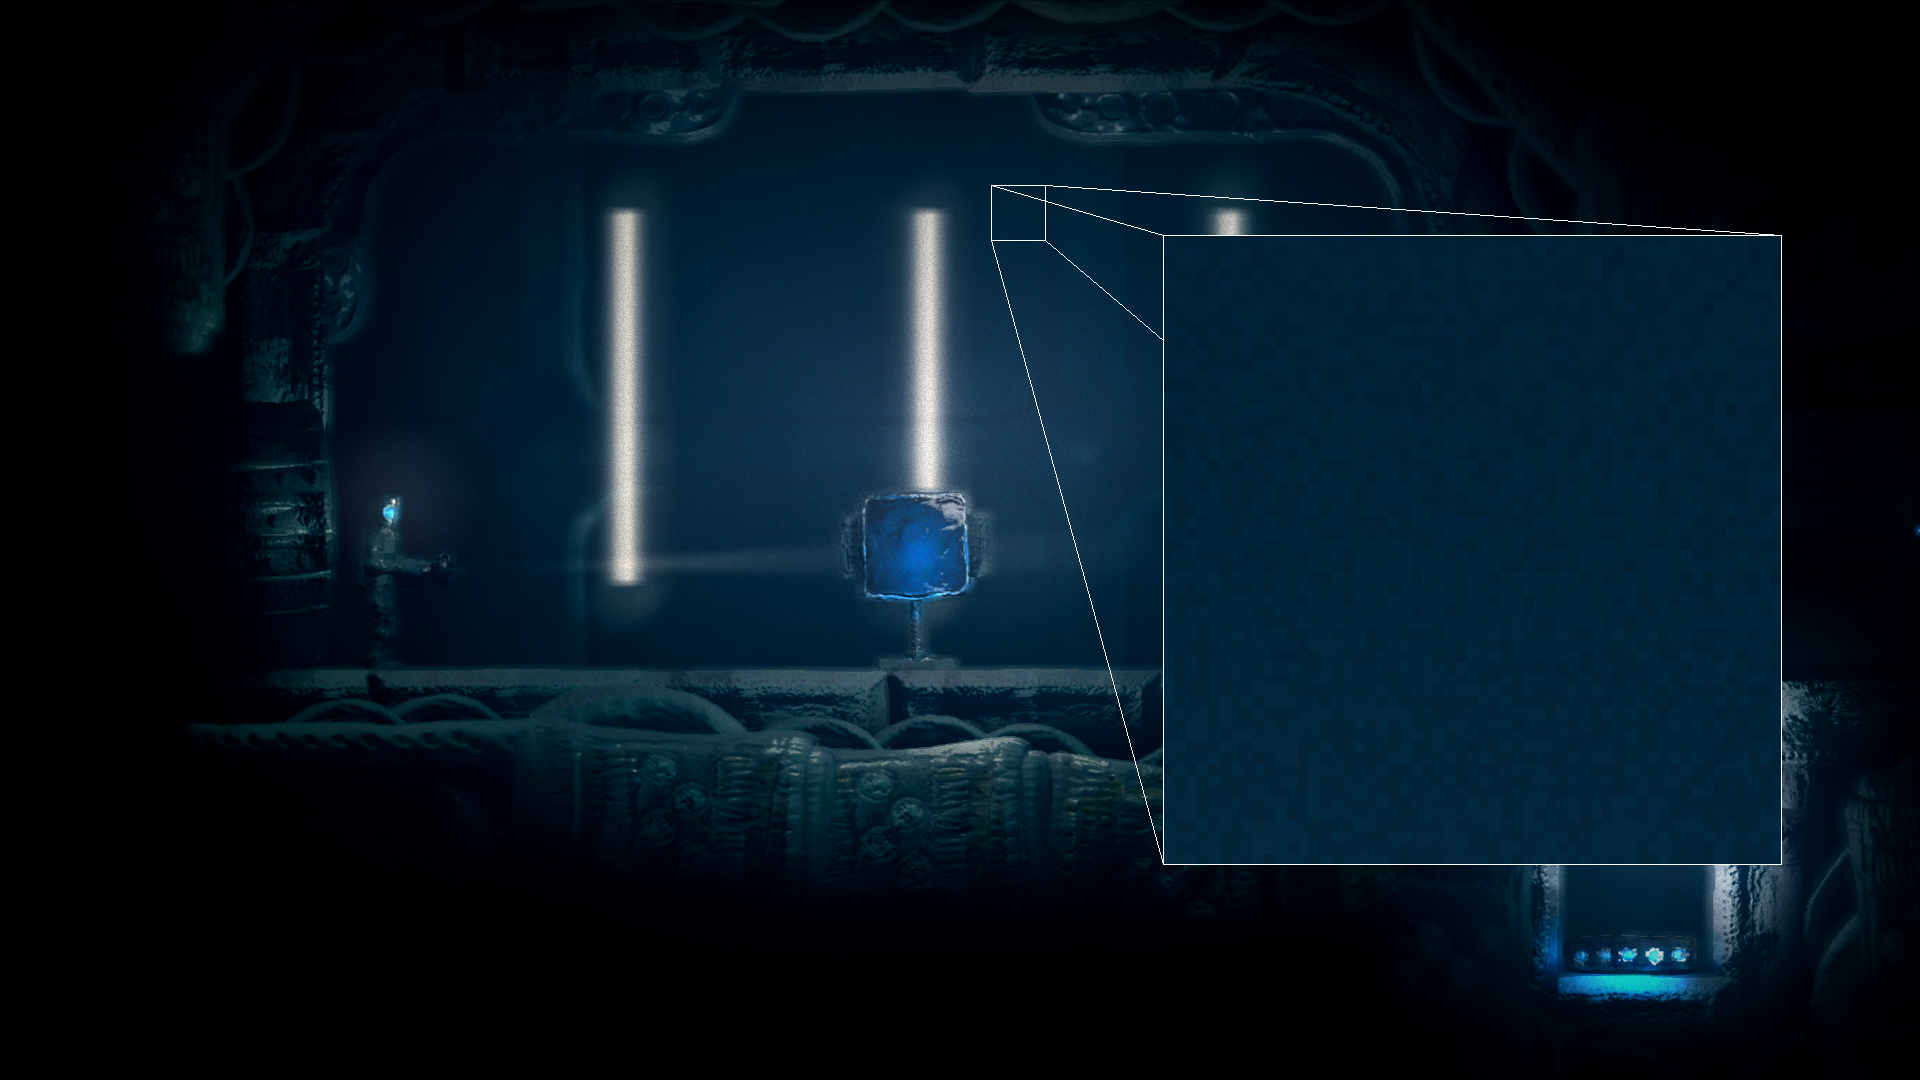
\includegraphics[scale=0.09]{TheSwapper.png}
			\vspace{-20px}
		\end{center}
		\caption{Film Grain in \textit{The Swapper}.}
		\begin{center}
			\vspace{-20px}
			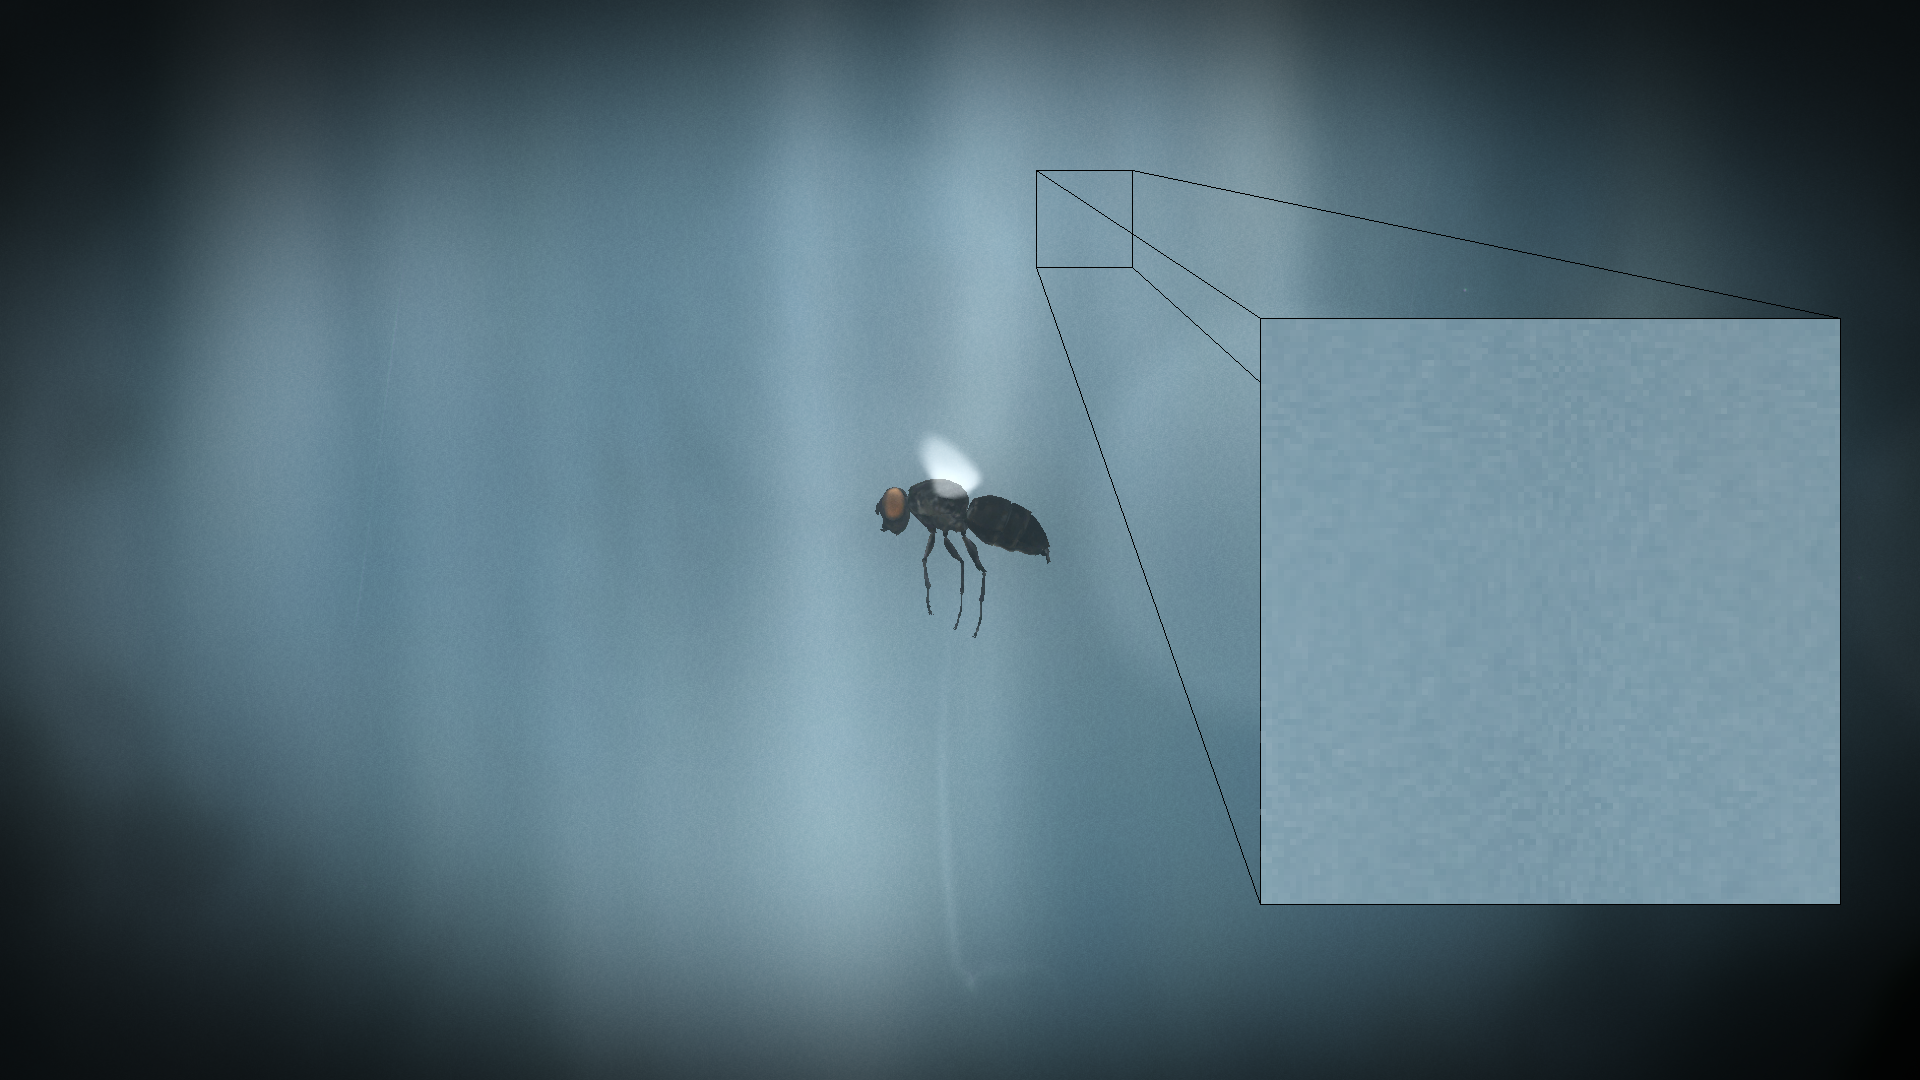
\includegraphics[scale=0.09]{ThePlan.png}
			\vspace{-20px}
		\end{center}
		\caption{Film Grain in \textit{The Plan}.}
	\end{wrapfigure}
	Film Grain can "roughen" these surfaces and makes the image look more interesting. As the grain nullifies itself in greater areas, the image is not affected negatively.
	
\end{document}